
%(BEGIN_QUESTION)
% Copyright 2011, Tony R. Kuphaldt, released under the Creative Commons Attribution License (v 1.0)
% This means you may do almost anything with this work of mine, so long as you give me proper credit

This air compressor control circuit has a problem.  The air compressor refuses to start even when the air pressure is zero PSI.  A technician begins diagnosing the circuit, following the steps shown (in order):

$$\includegraphics[width=15.5cm]{i03530x01.eps}$$

\begin{itemize}
\item{} {\bf Test 1:} Measured 120 VAC between points {\bf A} and {\bf C}, with ``Hand/Off/Auto'' switch in the ``Auto'' position.
\vskip 25pt
\item{} {\bf Test 2:} Measured 120 VAC between points {\bf A} and {\bf D}, with ``Hand/Off/Auto'' switch in ``Auto'' position.
\vskip 25pt
\item{} {\bf Test 3:} Measured 0 VAC between points {\bf E} and {\bf C}, with ``Hand/Off/Auto'' switch in ``Auto'' position.
\vskip 25pt
\item{} {\bf Test 4:} Jumpered points {\bf A} and {\bf B}, with ``Hand/Off/Auto'' switch in ``Auto'' position.  The motor did not start.
\vskip 25pt
\end{itemize}

Identify any useful information about the nature or location of the fault derived from the results of each test, in order of the tests performed.  If the test is not useful (i.e. provides no new information), mark it as such.  Assuming there is only one fault in the circuit, identify the location and nature of the fault as precisely as you can from the test results shown above.

\vfil 

\underbar{file i03530}
\eject
%(END_QUESTION)





%(BEGIN_ANSWER)

\begin{itemize}
\item{} {\bf Test 1:} Measured 120 VAC between points {\bf A} and {\bf C}, with ``Hand/Off/Auto'' switch in the ``Auto'' position.  {\it Proves there is 120 VAC control power available, that the fuse is good, and that the Hand/Off/Auto switch is passing power through to point A.}
\vskip 5pt
\item{} {\bf Test 2:} Measured 120 VAC between points {\bf A} and {\bf D}, with ``Hand/Off/Auto'' switch in ``Auto'' position.  {\it Proves there is an ``open'' fault somewhere between those points, in one of the two switches, and that we do not have any other ``open'' faults in the contactor coil circuit.}
\vskip 5pt
\item{} {\bf Test 3:} Measured 0 VAC between points {\bf E} and {\bf C}, with ``Hand/Off/Auto'' switch in ``Auto'' position.  {\it This is an unnecessary test, as we already know there is continuity through the overload contact.}
\vskip 5pt
\item{} {\bf Test 4:} Jumpered points {\bf A} and {\bf B}, with ``Hand/Off/Auto'' switch in ``Auto'' position.  The motor did not start.  {\it Combined with the results of previous tests, this test proves the ``open'' fault must lie between points B and D: namely the PSH.}
\end{itemize}

\vskip 10pt

{\bf The fault is an ``open'' high pressure switch (PSH), or in the wires connecting the PSH to points B and D.}

%(END_ANSWER)





%(BEGIN_NOTES)

\vskip 20pt \vbox{\hrule \hbox{\strut \vrule{} {\bf Virtual Troubleshooting} \vrule} \hrule}

This question is a good candidate for a ``Virtual Troubleshooting'' exercise.  Presenting the diagram to students, you first imagine in your own mind a particular fault in the system.  Then, you present one or more symptoms of that fault (something noticeable by an operator or other user of the system).  Students then propose various diagnostic tests to perform on this system to identify the nature and location of the fault, as though they were technicians trying to troubleshoot the problem.  Your job is to tell them what the result(s) would be for each of the proposed diagnostic tests, documenting those results where all the students can see.

During and after the exercise, it is good to ask students follow-up questions such as:

\begin{itemize}
\item{} What does the result of the last diagnostic test tell you about the fault?
\item{} Suppose the results of the last diagnostic test were different.  What then would that result tell you about the fault?
\item{} Is the last diagnostic test the best one we could do?
\item{} What would be the ideal order of tests, to diagnose the problem in as few steps as possible?
\end{itemize}


%INDEX% Troubleshooting review: electric circuit diagnostic test rationale

%(END_NOTES)


